\documentclass[12pt]{extarticle} 
\usepackage{amsmath}
\usepackage{amsmath}
\usepackage{array}
\usepackage{booktabs}  % For nicer rules

\usepackage{graphicx} % Required for inserting images
\usepackage{placeins}  % In preamble
\usepackage{geometry}


% Or set margins directly
\geometry{left=2.5cm, right=2.5cm, bottom=3cm, top=3cm}  % This also affects text width


\FloatBarrier  % Prevents figures from floating past this point
%
\usepackage[absolute,overlay]{textpos}  % In preamble
\title{Transformer Notes}
\author{Yue Wu}
\date{February 2026}

\begin{document}

\maketitle

\tableofcontents

\section{Attention Mechanism}
\begin{figure}[htbp]
    \centering
    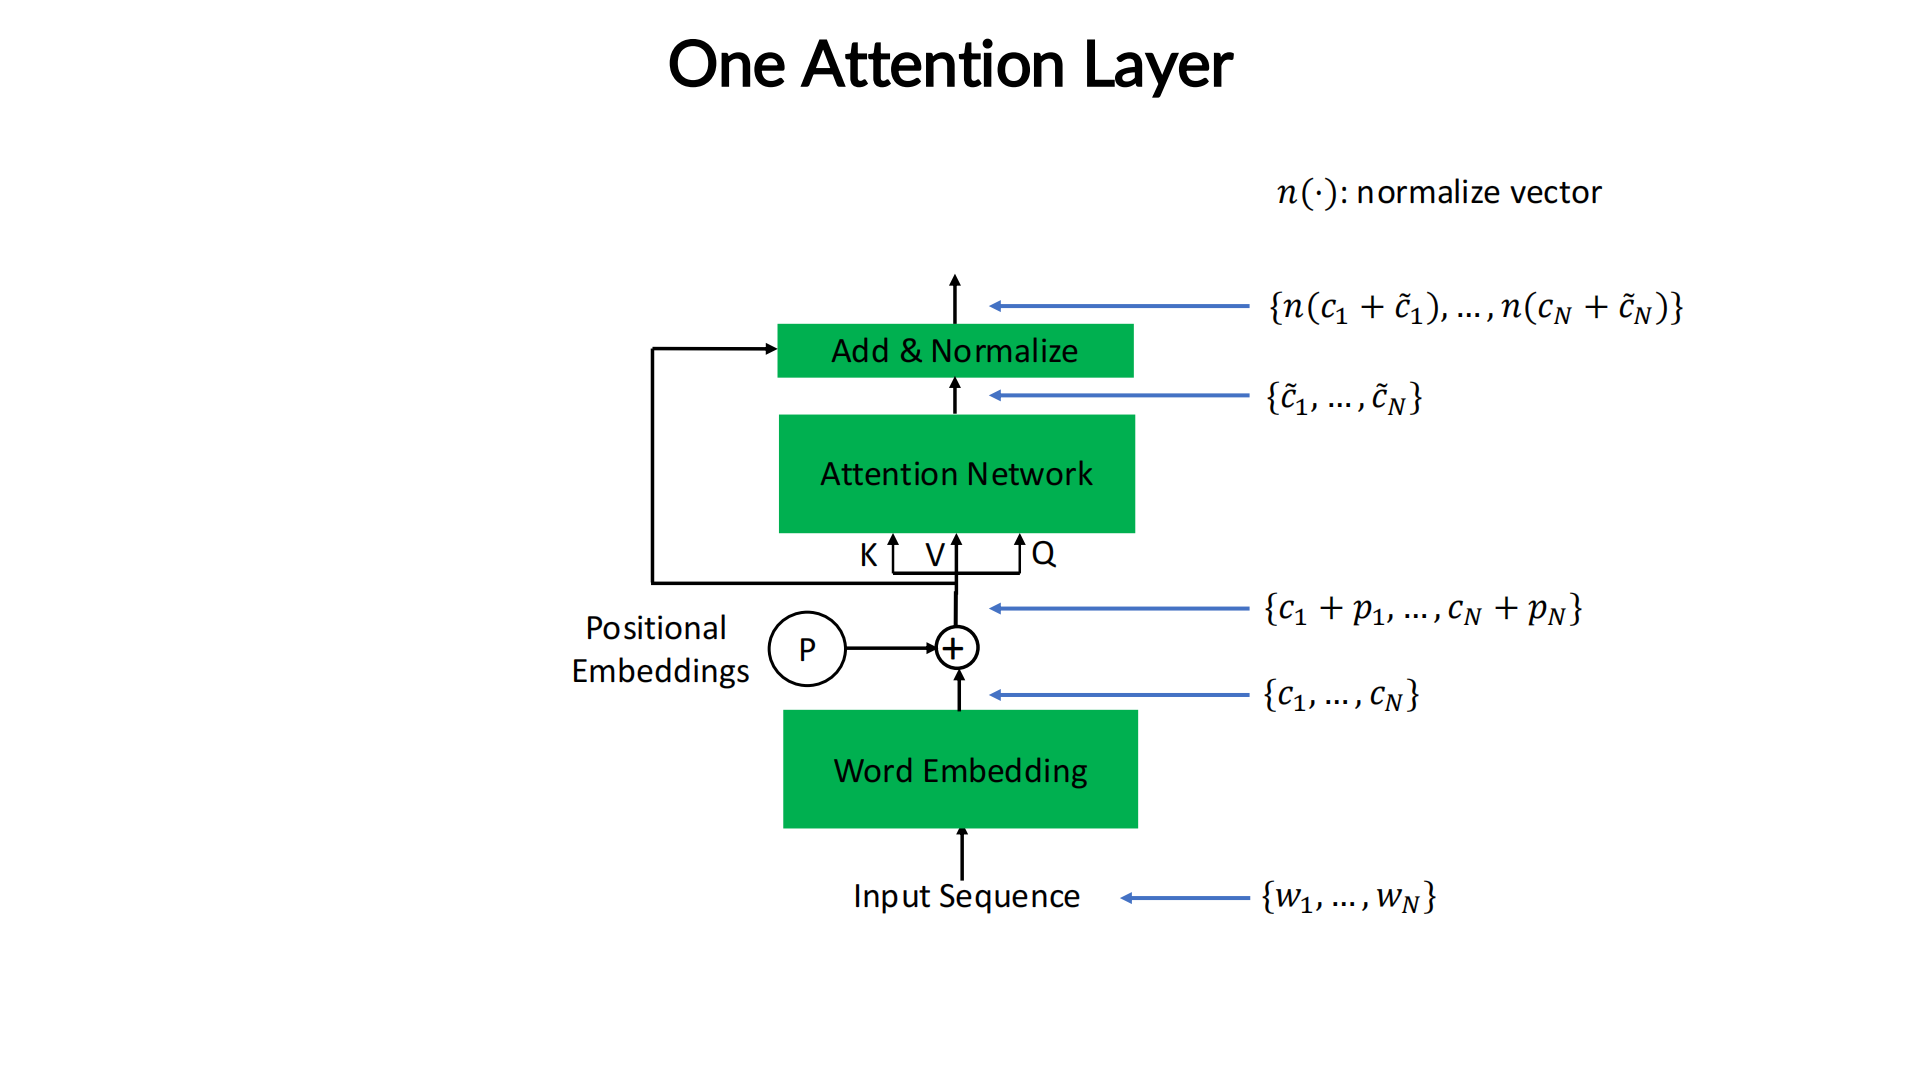
\includegraphics[width=0.8\textwidth]{untitled folder/ECE590_Lecture9_02.png}
    \caption{Attention}
\end{figure}
\FloatBarrier
\subsection*{1. Input Sequence}
The process begins with an input sequence of $N$ tokens:
\[
\text{Input} = [w_1, w_2, \ldots, w_N]
\]

\subsection*{2. Word Embedding}
Each token is mapped to a dense vector representation via word embeddings:
\[
\{c_1, c_2, \ldots, c_N\}, \quad c_i \in \mathbb{R}^d
\]
where $d$ is the embedding dimension.

\subsection*{3. Positional Embeddings}
Since Transformers have no inherent notion of word order, positional encodings are added:
\[
\{p_1, p_2, \ldots, p_N\}, \quad p_i \in \mathbb{R}^d
\]
These capture the position of each token in the sequence.

\subsection*{4. Combined Input to Attention}
The word embeddings and positional embeddings are summed to produce the input to the attention layer:
\[
 c_i + p_i, \quad \text{for } i = 1, \ldots, N
\]
Thus, the input to the attention network is:
\[
\{c_1+p_1, c_2+p_2, \ldots, c_N+p_N\}
\]

\subsection*{5. Attention Network}
The attention mechanism computes interactions between all positions. For each position $i$, it produces an output $\tilde{c}_i$ that is a weighted sum of values from all positions, where weights are determined by query-key similarities:
\[
\tilde{c}_i = \sum_{j=1}^N \text{Attention}(i,j) \cdot (W_V (c_j+p_j))
\]
The original input $c_i+p_i$ is not replaced; instead, we compute a residual update.

\subsection*{6. Skip Connection (Add)}
The original input $c_i+p_i$ is added back to the attention output:
\[
(c_i+p_i) + \tilde{c}_i
\]
This skip connection (residual connection) helps with gradient flow during training and preserves the original information.

\subsection*{7. Add \& Normalize}
Finally, layer normalization is applied to the sum:
\[
n((c_i+p_i) + \tilde{c}_i)
\]
where $n(\cdot)$ denotes vector normalization (typically layer norm). The output of the layer is:
\[
\{n(c_1+p_1 + \tilde{c}_1), n(c_2 +p_2+ \tilde{c}_2), \ldots, n(c_N +p_N + \tilde{c}_N)\}
\]

\subsection*{Summary}
\begin{itemize}
    \item \textbf{Input:} $\{c_i\}$ (word embeddings) $+$ $\{p_i\}$ (positional embeddings) $\rightarrow$ $\{c_i+p_i\}$
    \item \textbf{Attention:} Computes context vectors $\{\tilde{c}_i\}$ based on all positions
    \item \textbf{Skip connection:} $\{c_i  +p_i+\tilde{c}_i\}$ preserves original information
    \item \textbf{Normalization:} $\{n(c_i +p_i+ \tilde{c}_i)\}$ stabilizes training
    \item \textbf{Output:} Contextualized representations ready for the next layer
\end{itemize}

This architecture allows each token to gather information from the entire sequence while maintaining its own identity through the residual connection.


\begin{figure}[htbp]
    \centering
    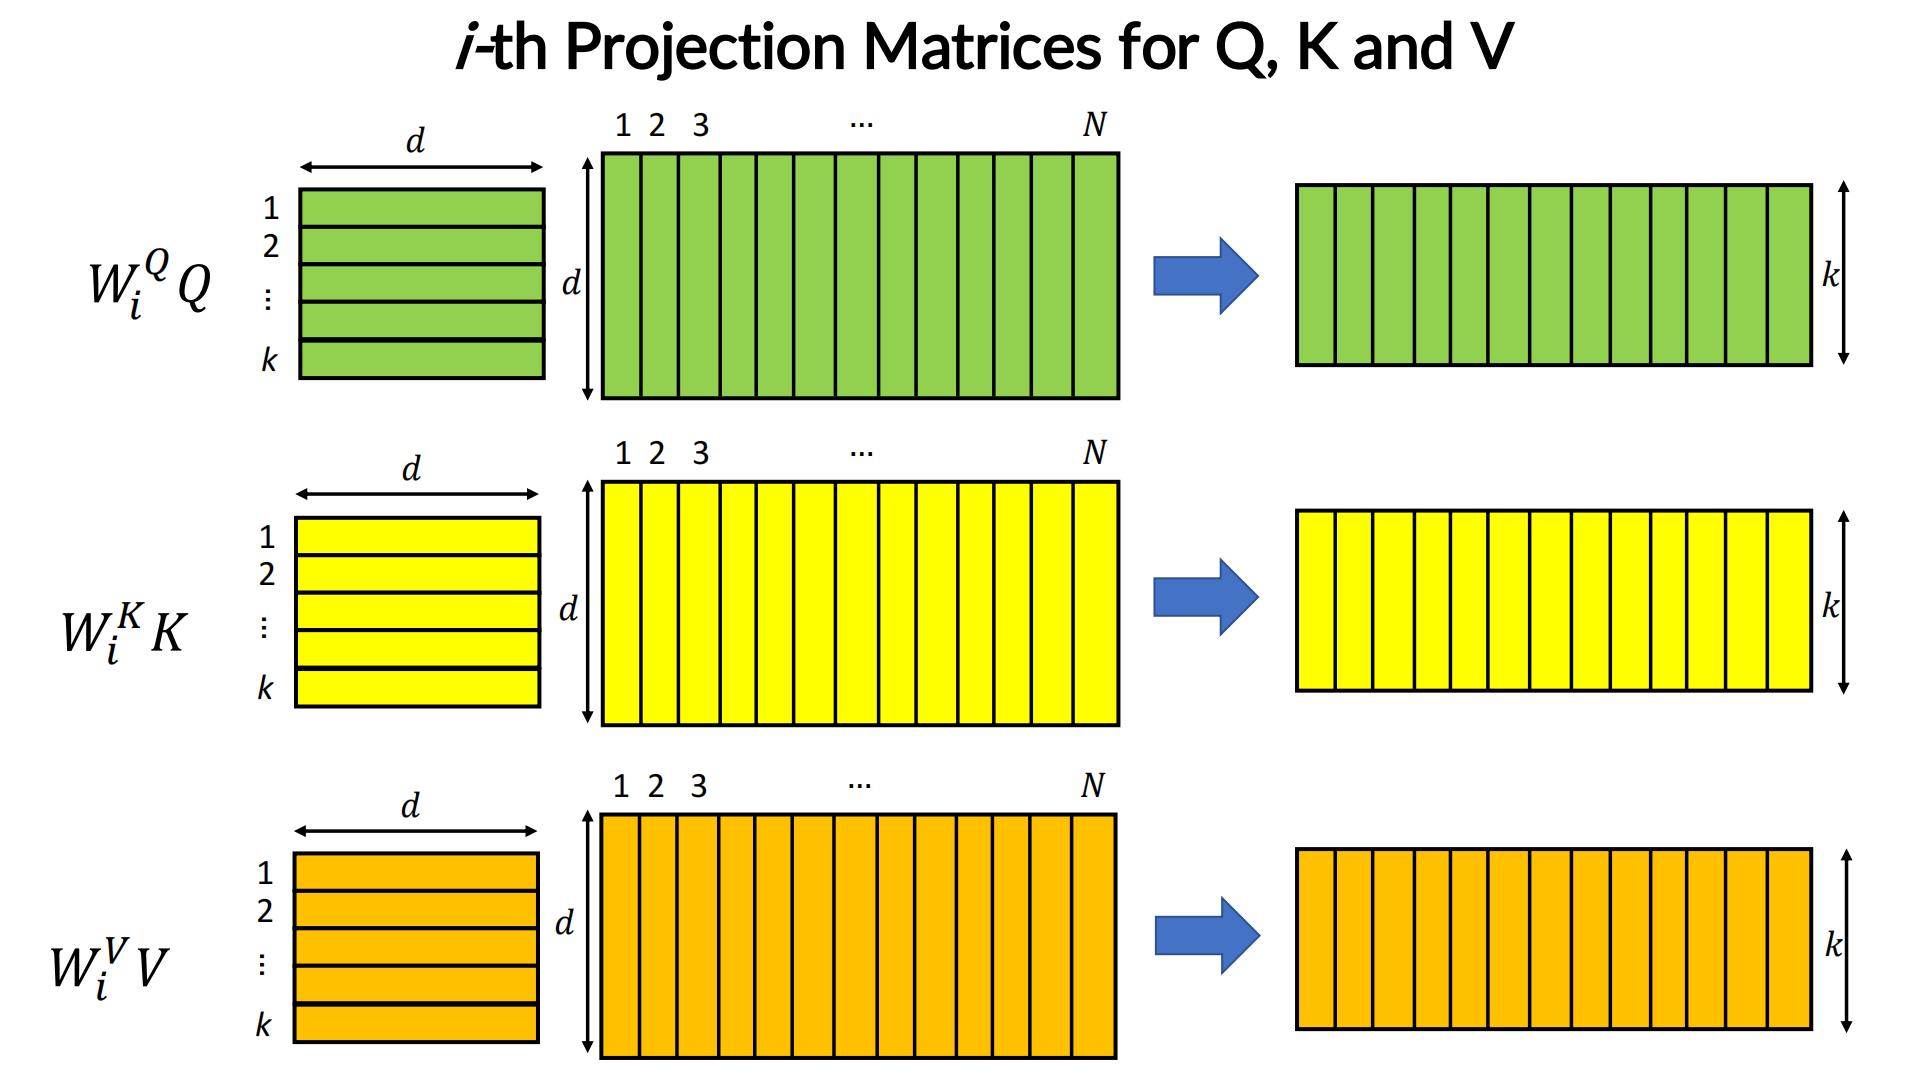
\includegraphics[width=0.6\textwidth]{untitled folder/ECE590_Lecture9_18.png}
    \caption{Attention}
\end{figure}
\FloatBarrier

In the figure above, each weight matrix like $W_i^Q$ is a matrix of dimension $d_k(64) \times d_{\text{model}}(512)$. $Q$ is a matrix of dimension $d_{\text{model}}(512) \times \text{sequence length}(n)$.
\begin{figure}[htbp]
    \centering
    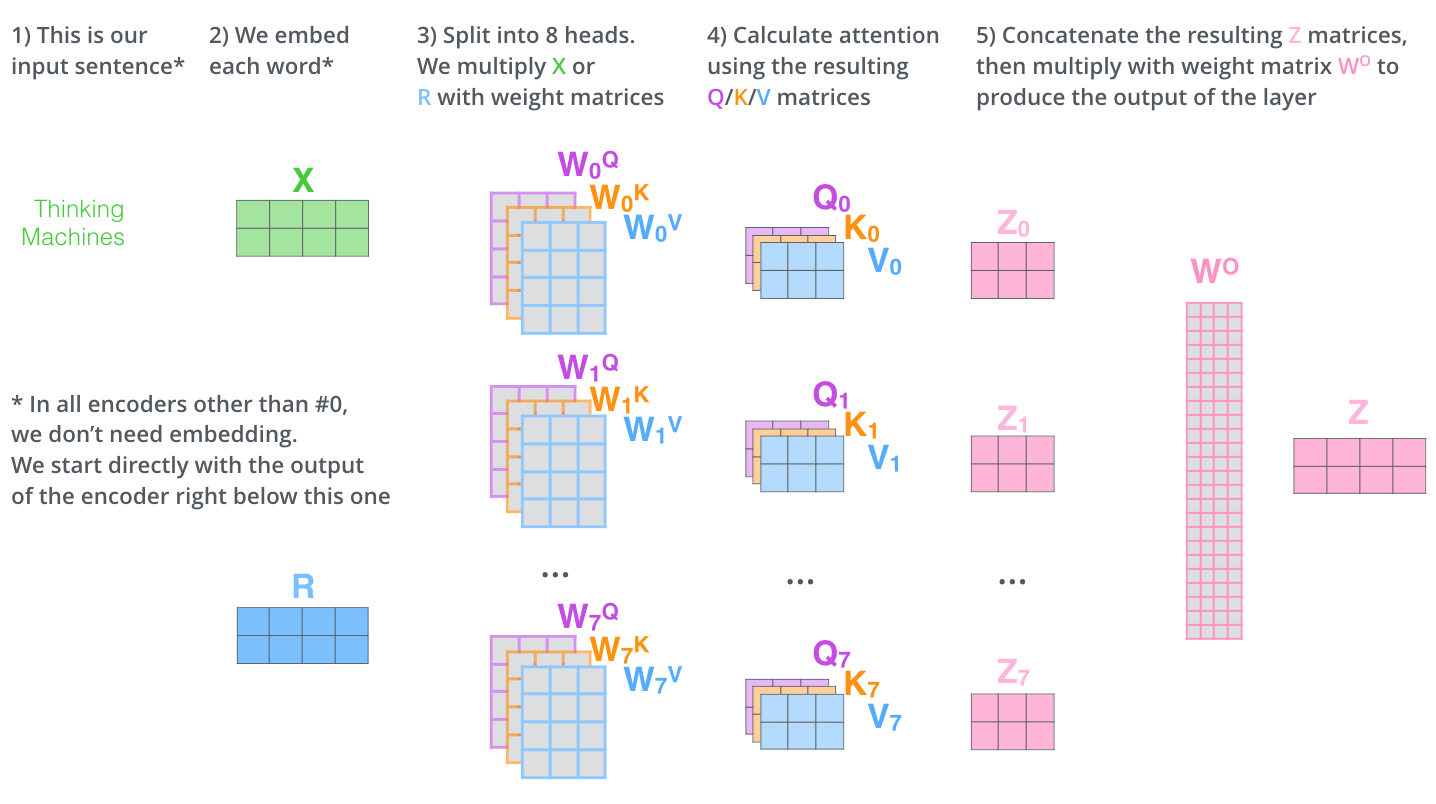
\includegraphics[width=0.7\textwidth]{transformer_multi-headed_self-attention-recap.png}
    \caption{Multihead Self Attention}
\end{figure}
\FloatBarrier

In the figure above, the input matrices were differentiated to Q,K,V, just to generalize to the cross attention. In self attention, they are the same.

$$\text{Multi-Headed Output} = \text{Concat}(\text{output}_1, \ldots, \text{output}_h) W^O,$$ $$ \text{ output}_i = \text{Attention}(W_i^K K, W_i^V V, W_i^Q Q)$$


The h projections associated with the multi-headed attention allow the model to attend based
on different aspects (projections) of the word vectors
Allows attention to focus on different aspects of the language/words
 Introduces many new parameters: the projection matrices
 
Recall the word embedding plus positional embedding, for word $n$ in the sequence:
\begin{itemize}
    \item For head $i$, the multi-head attention acts on this sum as (because of linearity):
    \[
    w_n = e_n + p_n
    \]
    \begin{align*}
    W_i^Q w_n &= W_i^Q e_n + W_i^Q p_n \\
    W_i^K w_n &= W_i^K e_n + W_i^K p_n \\
    W_i^V w_n &= W_i^V e_n + W_i^V p_n
    \end{align*}
\end{itemize}

For positional encoding: 

\begin{align*}
PE_{(pos, 2i)} &= \sin\left(\frac{pos}{10000^{2i/d}}\right) \\
PE_{(pos, 2i+1)} &= \cos\left(\frac{pos}{10000^{2i/d}}\right)
\end{align*}


\begin{enumerate}
    \item \textbf{Positional frequencies:} Recall that the positional embeddings have components that oscillate at different frequencies.
    
    \item \textbf{Proximity scaling:} The head matrices $W_i^Q$, $W_i^K$ and $W_i^V$ may be learned to emphasize different components of the positional embeddings, effectively setting a measure of scale of closeness (proximity).
    
    \item \textbf{Content emphasis:} The head matrices may also emphasize different components of $e_n$, thereby emphasizing particular topics or writing styles.
\end{enumerate}
\subsection{Examples}
\begin{align*}
W_i^Q w_n &= W_i^Q e_n + W_i^Q p_n \approx W_i^Q p_n \\
W_i^K w_n &= W_i^K e_n + W_i^K p_n \approx W_i^K p_n \\
W_i^V w_n &= W_i^V e_n + W_i^V p_n
\end{align*}

Direct particular attention to words nearby the next word to be predicted.

\begin{itemize}
    \item $W_i^Q$ and $W_i^K$ are designed (learned) such that $W_i^Q e_n \approx \mathbf{0}_d$ and $W_i^K e_n \approx \mathbf{0}_d$, where embeddings are of length $d$ and $\mathbf{0}_d$ is a $d$-dimensional vector of all zeros.
    
    \item $W_i^Q$ and $W_i^K$ are learned such that rows of these matrices emphasize components of $p_n$ that correspond to appropriate scales of positional ``closeness'' (recall components oscillate with position at a frequency that depends on the positional-encoding component).
\end{itemize}

\begin{align*}
W_i^Q w_n &= W_i^Q e_n + W_i^Q p_n \approx W_i^Q p_n \\
W_i^K w_n &= W_i^K e_n + W_i^K p_n \approx W_i^K p_n \\
W_i^V w_n &= W_i^V e_n + W_i^V p_n \approx W_i^V e_n
\end{align*}

\begin{itemize}
    \item $W_i^Q$ and $W_i^K$ are learned such that $W_i^Q e_n \approx \mathbf{0}_d$ and $W_i^K e_n \approx \mathbf{0}_d$, where $\mathbf{0}_d$ is a $d$-dimensional zero vector.
    
    \item $W_i^Q$ and $W_i^K$ are learned such that rows of these matrices emphasize components of $p_n$ that correspond to appropriate scales of positional ``closeness'' (recall components oscillate with position at a frequency that depends on the positional-encoding component).
    
    \item $W_i^V$ is learned such that $W_i^V p_n \approx \mathbf{0}_d$ and $W_i^V e_n \neq \mathbf{0}_d$, and rows of $W_i^V$ emphasize particular aspects of word meaning of ``most relevance'' when considering nearby words.
\end{itemize}

\begin{figure}[htbp]
    \centering
    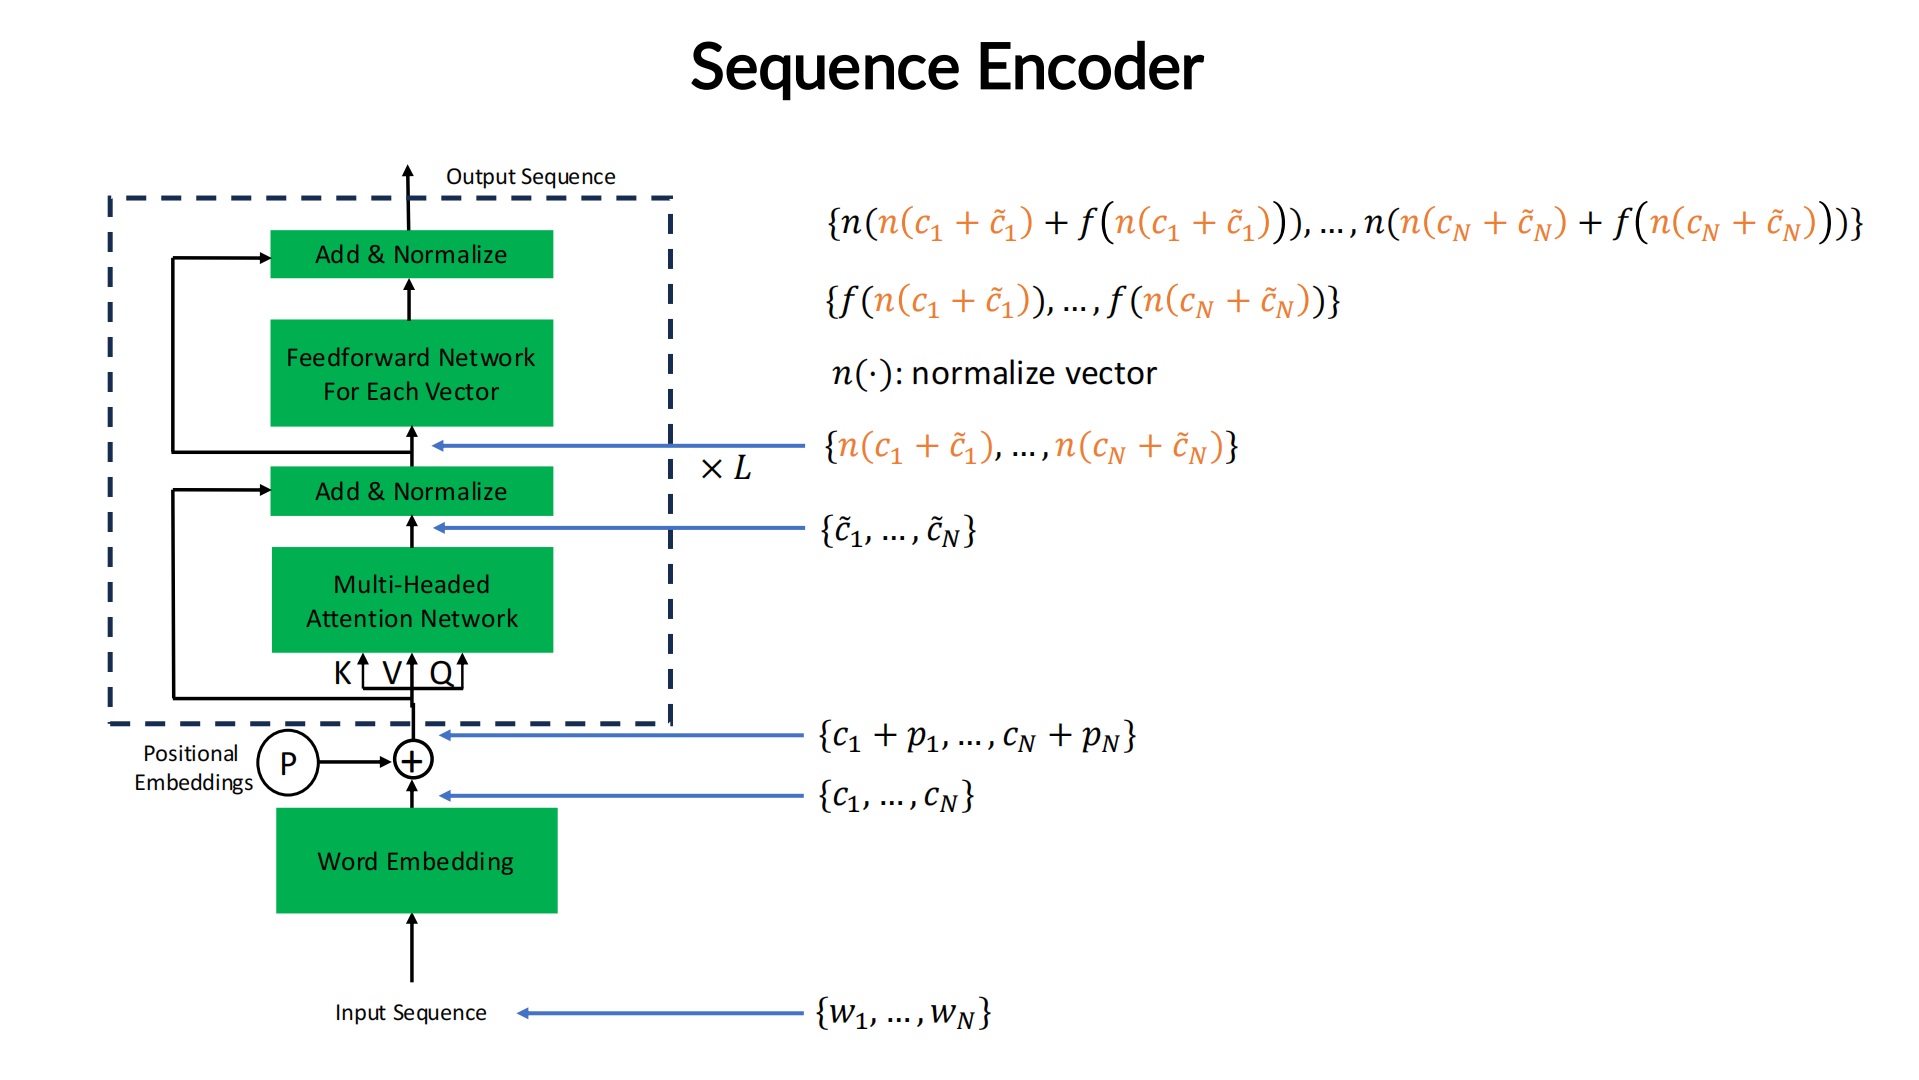
\includegraphics[width=0.7\textwidth]{untitled folder/ECE590_Lecture9_55.png}
    \caption{Encoder}
\end{figure}
\FloatBarrier

 \subsection*{Next Word Prediction}

The words for the prompt text are the first input sequence, consisting of $N$ tokens.

At the last layer $L$ of the network, we obtain output vectors
\[
\{f_1^{(L)}, f_2^{(L)}, \ldots, f_N^{(L)}\}
\]
corresponding to token positions $1$ through $N$, where the $N$-th word is the last in the sequence.

The objective is to predict the next word, i.e., the token at position $N+1$.

\begin{itemize}
    \item Recall that we have a set of learned embedding vectors $(w_1, \ldots, w_V)$ for the $V$ tokens in our vocabulary, with each $w_v \in \mathbb{R}^d$.
    
    \item Assume that $f_N^{(L)} \in \mathbb{R}^d$.
    
    \item Additional parameters manifested by matrix $M \in \mathbb{R}^{d \times d}$ acting after the last layer.
    
    \item Define the vector output $u = M f_N^{(L)}$.
\end{itemize}

Define the vector output $u = M f_N^{(L)}$.

The probability of token $v \in \{1, \ldots, V\}$ being the next word is modeled as
\[
p(v \mid \text{prompt}) = \frac{\exp[w_v^T u]}{\sum_{v'=1}^{V} \exp[w_{v'}^T u]}
\]

In autoregressive language models (like GPT), the attention mechanism is masked so tokens can only attend to themselves and previous tokens – never to future tokens.

The last token sees the information of previous tokens through stacks of masked attention layers. 

\subsection*{Training via Cross-Entropy Loss}

\begin{itemize}
    \item Let all Transformer parameters be represented as $\theta$, including the token embedding vectors.
    
    \item The probability of token $v \in \{1, \ldots, V\}$ is
    \[
    p_\theta(v \mid \text{prompt}) = \frac{\exp[w_v^T u]}{\sum_{v'=1}^{V} \exp[w_{v'}^T u]}
    \]
    
    \item Assume we have a collection of text prompts $\{\text{prompt}^{(j)}\}_{j=1}^{J}$ and let $w_{N+1}^{(j)}$ represent the true next word connected to prompt $j$.
    
    \item Learn $\theta$ by seeking to minimize the cross-entropy loss for prediction of the next word.
\end{itemize}

\[
\hat{\theta} = \arg\min_{\theta} \left[ -\sum_{j=1}^{J} \log p_{\theta}\left(v = w_{N+1}^{(j)} \;\big|\; \text{prompt}^{(j)}\right) \right]
\]

Design the Transformer parameters such that the model has a high likelihood of predicting the true next word, across all prompts in the corpus.


\section*{The Feedforward Layer in Transformers}

The feedforward layer (FFN) is a crucial component in each Transformer block, positioned after the multi-head attention mechanism.

\subsection*{1. Architecture Overview}

Within a single Transformer block, the feedforward layer appears as:

\[
\text{Input} \rightarrow \text{Multi-Head Attention} \rightarrow \text{Add \& Norm} \rightarrow \boxed{\text{Feedforward}} \rightarrow \text{Add \& Norm} \rightarrow \text{Next Layer}
\]

\subsection*{2. Mathematical Formulation}

For a single position vector $\mathbf{x} \in \mathbb{R}^{d_{\text{model}}}$, the feedforward layer computes:

\[
\text{FFN}(\mathbf{x}) = W_2 \cdot \text{Activation}(W_1 \mathbf{x} + b_1) + b_2
\]

where:
\begin{itemize}
    \item $W_1 \in \mathbb{R}^{d_{\text{ff}} \times d_{\text{model}}}$, $b_1 \in \mathbb{R}^{d_{\text{ff}}}$ (first layer)
    \item $W_2 \in \mathbb{R}^{d_{\text{model}} \times d_{\text{ff}}}$, $b_2 \in \mathbb{R}^{d_{\text{model}}}$ (second layer)
    \item Activation function: typically ReLU or GELU
    \item $d_{\text{ff}}$ is usually $4 \times d_{\text{model}}$ (e.g., 2048 vs 512)
\end{itemize}

\subsection*{3. Common Activation Functions}

\[
\text{ReLU}(x) = \max(0, x)
\]

\[
\text{GELU}(x) = x \cdot \Phi(x) \quad \text{where } \Phi(x) \text{ is the standard Gaussian CDF}
\]

\subsection*{4. Key Properties}

\begin{table}[h]
\centering
\begin{tabular}{lp{10cm}}
\toprule
\textbf{Property} & \textbf{Description} \\
\midrule
Position-wise & Applied independently to each token position \\
Two-layer & Expands dimension then compresses back \\
Nonlinear & Activation function introduces nonlinearity \\
Identical weights & Same $W_1, W_2$ used for all positions \\
Layer-specific & Each Transformer layer has its own FFN weights \\
\bottomrule
\end{tabular}
\end{table}

\subsection*{5. The Expansion Factor}

A typical configuration:

\[
d_{\text{model}} = 512, \quad d_{\text{ff}} = 2048 \quad (\text{4× expansion})
\]

\[
W_1: 512 \rightarrow 2048 \quad \text{(expand)}
\]
\[
\text{Activation: ReLU/GELU} \quad \text{(nonlinear)}
\]
\[
W_2: 2048 \rightarrow 512 \quad \text{(compress)}
\]

\subsection*{6. What Does It Do? (Intuitions)}

\begin{itemize}
    \item \textbf{Memory Storage:} Stores factual knowledge (key-value memory view)
    \item \textbf{Feature Transformation:} Processes information gathered by attention
    \item \textbf{Pattern Completion:} Completes patterns partially activated by attention
    \item \textbf{Nonlinear Computation:} Essential for complex tasks (attention alone is linear)
\end{itemize}

\subsection*{7. Attention vs. Feedforward}

\begin{table}[h]
\centering
\begin{tabular}{lcc}
\toprule
\textbf{Aspect} & \textbf{Attention} & \textbf{Feedforward} \\
\midrule
Communication & Across positions & Within position only \\
Operation & Weighted sum of values & Dense neural network \\
Parameters & Q, K, V matrices & Two weight matrices \\
Role & Information gathering & Information processing \\
Linearity & Linear (weighted sum) & Nonlinear (activation) \\
\bottomrule
\end{tabular}
\end{table}

\subsection*{8. The Complete Pattern}

\[
\boxed{\text{Gather} \rightarrow \text{Process}}
\]

\begin{align*}
\text{Attention:} & \quad \text{Gather information from other positions} \\
\text{Feedforward:} & \quad \text{Process that information at current position}
\end{align*}

\subsection*{9. Mathematical Example}

For a single position $i$ at layer $l$:

\[
\mathbf{x}_i^{(l)} = \text{LayerNorm}\left(\mathbf{x}_i^{(l-1)} + \text{Attention}(\mathbf{x}_i^{(l-1)})\right)
\]

\[
\mathbf{x}_i^{(l+1)} = \text{LayerNorm}\left(\mathbf{x}_i^{(l)} + W_2 \cdot \text{GELU}(W_1 \mathbf{x}_i^{(l)} + b_1) + b_2\right)
\]

\subsection*{10. Summary}

\begin{itemize}
    \item \textbf{What:} Two-layer neural network applied per position
    \item \textbf{Why:} Adds nonlinearity and processing capacity
    \item \textbf{How:} Expands dimension, applies activation, compresses back
    \item \textbf{Size:} Typically 4× expansion of dimension
    \item \textbf{Location:} After attention in each Transformer block
\end{itemize}

In one sentence: \textit{The feedforward layer is where each token individually processes and refines the information gathered by attention, adding essential nonlinearity and accessing stored knowledge.}

\section{Encoder-Decoder Architecture}
\begin{figure}[htbp]
    \centering
    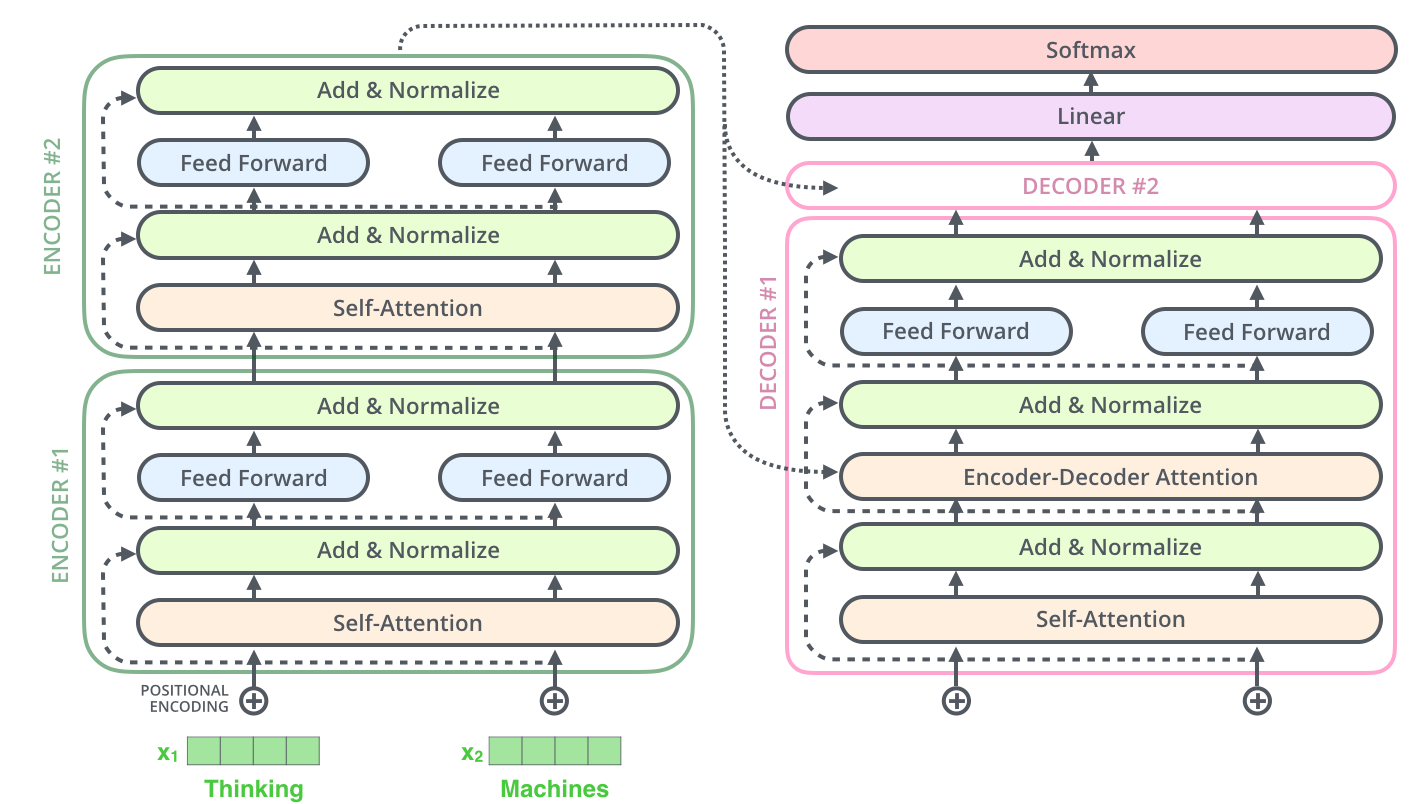
\includegraphics[width=0.7\textwidth]{transformer_resideual_layer_norm_3.png}
    \caption{Encoder-Decoder}
\end{figure}
\FloatBarrier


The transformer consists of two main components:

\begin{itemize}
\item \textbf{Encoder:} Builds a contextual understanding of the input sequence.
\item \textbf{Decoder:} Generates the output sequence using the encoder's representation and the previously generated tokens (starting with \texttt{<BOS>}).
\end{itemize}

\subsection{Encoder}

Given an input sequence \( X \in \mathbb{R}^{T \times d} \), the encoder processes it through multiple identical layers. Each layer contains:

\begin{enumerate}
\item \textbf{Self-Attention:}  
Each token attends to all other tokens, allowing the model to capture contextual relationships.

\[
\text{Attention}(Q,K,V) = \text{softmax}\left(\frac{QK^T}{\sqrt{d_k}}\right)V
\]

\[
\text{Attention}(Q,K,V) =
\text{softmax}\left(\frac{QK^T}{\sqrt{d_k}}\right)V
\]

In self-attention, the queries, keys, and values are computed from the same input matrix \(X\), but with different learned projection matrices:

\[
Q = XW_Q
\]

\[
K = XW_K
\]

\[
V = XW_V
\]

where

\[
W_Q,\; W_K,\; W_V \in \mathbb{R}^{d_{\text{model}} \times d_k}.
\]

Equivalently, self-attention can be written compactly as:

\[
\text{SelfAttention}(X)
=
\text{softmax}
\left(
\frac{(XW_Q)(XW_K)^T}{\sqrt{d_k}}
\right)
(XW_V).
\]

\item \textbf{Feedforward Network:}  
Applies a position-wise nonlinear transformation to each token independently.

\end{enumerate}

After several layers, the encoder produces a contextual representation:

\[
E = \text{Encoder}(X), \quad E \in \mathbb{R}^{T \times d}
\]

This representation acts as a \textbf{memory} of the input sequence.

\subsection{Decoder}

The decoder generates tokens autoregressively (one at a time). Each decoder layer has three components:

\begin{enumerate}

\item \textbf{Masked Self-Attention:}  
Allows each position to attend only to previously generated tokens, preventing access to future information.

\item \textbf{Cross-Attention (Encoder--Decoder Attention):}  

This is the key interaction between encoder and decoder.

\[
Q = \text{decoder states}, \quad K,V = E
\]

The decoder queries the encoder representation to retrieve relevant information for predicting the next token.

\item \textbf{Feedforward Network:}  
Further transforms the combined information.

\end{enumerate}

\subsection*{Information Flow}

\[
\text{Input Tokens} \rightarrow \text{Encoder} \rightarrow E
\]

\[
\text{Previous Outputs} + E \rightarrow \text{Decoder} \rightarrow \text{Next Token}
\]


\subsection*{Key Insights}

\begin{itemize}
\item The encoder does not generate text; it builds a structured understanding.
\item The decoder repeatedly attends to the encoder output at every layer.
\item Cross-attention removes the information bottleneck found in older sequence-to-sequence models.
\item Both components are trained jointly so the encoder learns representations that are useful for the decoder.
\end{itemize}

\subsection*{Conceptual Summary}

\begin{center}
\textbf{Encoder understands $\quad \rightarrow \quad$ Decoder generates}
\end{center}

Or equivalently:

\begin{center}
\textit{Comprehension $\rightarrow$ Guided Generation}
\end{center}







\section{Encoder Details}
Assume that we have $N$ inputs, and let $e_i^{(0)} \in \mathbb{R}^d$ represent the vector at position $i = 1, \ldots, N$ input to attention layer $l = 1$.

\begin{itemize}
    \item Simplify by considering only one attention head, with parameters $W_Q \in \mathbb{R}^{d \times d}$, $W_K \in \mathbb{R}^{d \times d}$, $W_V \in \mathbb{R}^{d \times d}$ and $P \in \mathbb{R}^{d \times d}$.
    
    \item Assume $W_Q$, $W_K$, $W_V$ and $P$ are the same at all attention layers (simplification).
\end{itemize}

The output at position $i$ from first attention layer, plus skip connection, is
\[
e_i^{(1)} = e_i^{(0)} + P \sum_{j=1}^{N} (W_V e_j^{(0)}) w_{ij}^{(0)}
\]
where
\[
w_{ij}^{(0)} = \frac{\exp\left[\lambda (W_Q e_i^{(0)})^T (W_K e_j^{(0)})\right]}{\sum_{j'=1}^{N} \exp\left[\lambda (W_Q e_i^{(0)})^T (W_K e_{j'}^{(0)})\right]}
\]



\subsection{Part 1: The Update Rule}
\[
e_i^{(1)} = e_i^{(0)} + P \sum_{j=1}^{N} (W_V e_j^{(0)}) w_{ij}^{(0)}
\]

\begin{table}[h]
\centering
\begin{tabular}{>{\tt}l l p{8cm}}
\toprule
\multicolumn{1}{c}{Symbol} & Meaning & \multicolumn{1}{c}{Interpretation} \\
\midrule
$e_i^{(0)}$ & Input vector at position $i$ (before attention) & The initial representation of word $i$ (e.g., ``bank'' could mean river or money) \\
$e_i^{(1)}$ & Output vector at position $i$ (after attention) & The \textbf{contextualized} representation after seeing the whole sentence \\
$P$ & Projection matrix (learned) & ``How much should I revise my understanding based on context?'' \\
$W_V e_j^{(0)}$ & Value of position $j$ & The \textbf{semantic content} of word $j$ — what information it contributes \\
$w_{ij}^{(0)}$ & Attention weight from $i$ to $j$ & How \textbf{relevant} is word $j$ to understanding word $i$? \\
$\sum_{j=1}^{N}$ & Sum over all positions $j$ & Consider \textbf{every word} in the sentence, weighted by relevance \\
\bottomrule
\end{tabular}
\caption{Update Rule for Attention with Skip Connection}
\end{table}

\subsection{Part 2: The Attention Weights}
\[
w_{ij}^{(0)} = \frac{\exp\left[\lambda (W_Q e_i^{(0)})^T (W_K e_j^{(0)})\right]}{\sum_{j'=1}^{N} \exp\left[\lambda (W_Q e_i^{(0)})^T (W_K e_{j'}^{(0)})\right]}
\]

\begin{table}[h]
\centering
\begin{tabular}{>{\tt}l l p{8cm}}
\toprule
\multicolumn{1}{c}{Symbol} & Meaning & \multicolumn{1}{c}{Interpretation} \\
\midrule
$W_Q e_i^{(0)}$ & \textbf{Query} of word $i$ & What \textbf{information} is word $i$ looking for? (e.g., ``I need to know the subject'') \\
$W_K e_j^{(0)}$ & \textbf{Key} of word $j$ & What \textbf{information} does word $j$ offer? (e.g., ``I am a noun'') \\
$(W_Q e_i)^T (W_K e_j)$ & \textbf{Similarity score} & How well does word $j$'s content \textbf{match} what word $i$ needs? \\
$\lambda$ & Scaling factor & Controls how \textbf{selective} the attention is \\
Denominator & Sum over all $j$ & Ensures all attention weights \textbf{add up to 1} \\
\bottomrule
\end{tabular}
\caption{Attention Weights via Softmax}
\end{table}


\newpage
The output at position $i$ from first attention layer, plus skip connection, is
\[
e_i^{(1)} = e_i^{(0)} + P \sum_{j=1}^{N} (W_V e_j^{(0)}) w_{ij}^{(0)}
\]

\begin{itemize}
    \item The weight $w_{ij}^{(0)}$ is a measure of how much ``attention'' should be placed on position $j$, when updating vector at position $i$.
    
    \item Let's simplify this: Let
    \[
    w_{ij}^{(0)} = (W_Q e_i^{(0)})^T (W_K e_j^{(0)}) = (e_i^{(0)})^T W_Q^T W_K e_j^{(0)} = (e_i^{(0)})^T \Phi e_j^{(0)}
    \]
\end{itemize}

Further simplify the setup such that $\Phi$ is the identity matrix.

\begin{itemize}
    \item The update rule for layer one plus skip connection is now
    \[
    e_i^{(1)} = e_i^{(0)} + P \sum_{j=1}^{N} (W_V e_j^{(0)}) \underbrace{\left[(e_i^{(0)})^T e_j^{(0)}\right]}_{\text{linear attention}}
    \]
    
    \item A simplification, but captures most elements of the attention network, plus skip connection.
\end{itemize}

The update rule for layer $l = 1, \ldots, L$, plus skip connections, is now
\[
e_i^{(l)} = e_i^{(l-1)} + P \sum_{j=1}^{N} (W_V e_j^{(l-1)}) \left[(e_i^{(l-1)})^T e_j^{(l-1)}\right]
\]

\begin{itemize}
    \item Have assumed, for simplicity, that $W_Q$, $W_K$, $W_V$ and $P$ are the same at all layers (need not be so in general).
\end{itemize}

Define the matrix $E_l = (e_1^{(l)}, \ldots, e_N^{(l)}) \in \mathbb{R}^{d \times N}$.

\begin{itemize}
    \item In matrix form, the update rule for all $N$ positions may be expressed
    \[
    E_l = E_{l-1} + P \underbrace{W_V E_{l-1}}_{\text{Values}} \underbrace{[E_{l-1}^T E_{l-1}]}_{\text{Attention}}
    \]
    
    \item Given context (``prompt'') associated with the $N$ inputs, predict the next sample $N+1$.
    
    \item The $N$ inputs are viewed as the context, or examples.
    
    \item Termed few-shot learning: The $N$ samples are contextual examples, and based on them predict $N+1$.
\end{itemize}

Given context (``prompt'') associated with the $N$ inputs, predict the next sample $N+1$.

\begin{itemize}
    \item The $N$ inputs are viewed as the context, or examples.
    
    \item Termed few-shot learning: The $N$ samples are contextual examples, and based on them predict $N+1$.
\end{itemize}

Few-shot learning is a widely studied field in machine learning.

\begin{itemize}
    \item Consider contextual data $C = \{(x_i, y_i)\}_{i=1}^N$, where $x_i \in \mathbb{R}^d$ and $y_i \in \mathbb{R}$.
    
    \item Assume that there is an unknown function $f(x) = y$ responsible for the outcomes: $y_i = f(x_i)$.
    
    \item Given the context $C$, infer the latent function $f(x)$, and use the inferred function to predict an outcome $y_{N+1} = f(x_{N+1})$ for a ``query'' $x_{N+1}$.
\end{itemize}

Few-shot learning has also been termed meta learning.

\begin{itemize}
    \item Wish to learn a meta model, that is able to adapt to new context, and make predictions that are context-dependent.
    
    \item Ideally, once we learn the meta model, its parameters do not change as it subsequently adapts to new context.
    
    \item Train the meta model such that it is capable of continuing to adapt, without parameter change.
    
    \item Overall goal: Learning to learn.
\end{itemize}

Consider training data composed of $M$ sets of contextual data, $C_m$, for $m = 1, \ldots, M$, where
\[
C_m = \{(x_i^{(m)}, y_i^{(m)})\}_{i=1}^{N+1}
\]

\begin{itemize}
    \item Train the meta model to take in context $\{(x_i^{(m)}, y_i^{(m)})\}_{i=1}^{N}$ and the query $x_{N+1}^{(m)}$.
    
    \item The meta model should be able to predict $y_{N+1}^{(m)}$ given the context and the query.
\end{itemize}

Let the Transformer be represented symbolically as $T_{\phi}(z)$, where $\phi$ are the Transformer parameters and $z$ represents the input set of vectors.

\begin{itemize}
    \item For context $m$, encode $\{(x_i^{(m)}, y_i^{(m)})\}_{i=1}^{N}$ and the query $x_{N+1}^{(m)}$ as $z$, and then use the Transformer to predict $y_{N+1}^{(m)}$.
    
    \item View the Transformer (here only in terms of attention and skip connection) as a meta learner.
    
    \item Once a Transformer has been trained, it can adapt to new prompts, with no change of Transformer parameters.
\end{itemize}

Consider contextual data
\[
C_m = (x_1^{(m)}, y_1^{(m)}, \ldots, x_N^{(m)}, y_N^{(m)})
\]
with $y_i^{(m)} = f_{\theta_m}(x_i^{(m)})$.

\begin{itemize}
    \item We now focus on linear model, $f_{\theta_m}(x) = w_m^T x$ where $\theta_m = w_m \in \mathbb{R}^d$.
    
    \item For example, we may assume each $w_m \sim \mathcal{N}(0_d, I_d)$.
    
    \item Also, may assume all covariates drawn $x_i^{(m)} \sim \mathcal{N}(0_d, I_d)$.
\end{itemize}

For the $m$th contextual dataset
\[
C_m = (x_1^{(m)}, y_1^{(m)}, \ldots, x_N^{(m)}, y_N^{(m)})
\]
assume a linear model, $f_{\theta_m}(x) = w_m^T x$ where $w_m \in \mathbb{R}^d$.

\begin{itemize}
    \item The latent $w_m$ is different for each set of contextual data.
    
    \item Can we train a meta model (the attention model) to take $C_{M+1}$ as input, along with the query $x_{N+1}^{(M+1)}$, and to predict $y_{N+1}^{(M+1)}$ for an underlying $w_{M+1}$ it has never seen?
    
    \item The trained model is trained such that it can perform inference based on a few examples (few-shot learning).
\end{itemize}

Hypothesis: Maybe the attention-based model can learn to perform gradient descent in its forward pass, based on the observed contextual data.

Cost function:
\[
\mathcal{L}(w) = \frac{1}{2} \sum_{i=1}^{N} (y_i - w^T x_i)^2
\]
where we have removed subscript $m$ for simplicity.

Gradient descent update:
\[
w_{k+1} = w_k + \alpha \sum_{i=1}^{N} (y_i - w_k^T x_i) x_i
\]
for gradient-descent step $k \geq 0$.

\begin{itemize}
    \item If $y_i - w_k^T x_i > 0$ then the model weights $w_k$ are putting too little emphasis in the direction of $x_i$.
    
    \item Hence, if $y_i - w_k^T x_i > 0$, then add positive weighting in direction of $x_i$: $\alpha(y_i - w_k^T x_i) x_i$ added to $w_k$ when updating.
    
    \item $\alpha$ is the learning rate.
    
    \item Similar if $y_i - w_k^T x_i < 0$, then subtract from $w_k$ vector in direction of $x_i$.
\end{itemize}

Using
\[
w_{k+1} = w_k + \alpha \sum_{i=1}^{N} (y_i - w_k^T x_i) x_i
\]
the model is updated as
\[
f_{\theta_{k+1}}(x_j) = w_k^T x_j + \alpha \sum_{i=1}^{N} (y_i - w_k^T x_i) x_j^T x_i = f_{\theta_k}(x_j) + \alpha \sum_{i=1}^{N} [y_i - f_{\theta_k}(x_i)] x_j^T x_i
\]

The update rule for GD with linear model is
\[
f_{\theta_{k+1}}(x_j) = f_{\theta_k}(x_j) + \alpha \sum_{i=1}^{N} [y_i - f_{\theta_k}(x_i)] x_j^T x_i
\]

\begin{itemize}
    \item Recall the update rule for linear attention:
    \[
    e_{j,k+1} = e_{j,k} + P[W_V E][E^T e_{j,k}]
    \]
    
    \item Can we construct $P$, $W_V$, $\Phi$ and the form of $e_i$ such that we achieve an equivalence?
\end{itemize}

Given context $C = (x_1, y_1, \ldots, x_N, y_N)$ and a query $x_{N+1}$.

\begin{itemize}
    \item GD update rule:
    \[
    \begin{aligned}
    f_{\theta_{k+1}}(x_j) &= f_{\theta_k}(x_j) + \alpha \sum_{i=1}^N [y_i - f_{\theta_k}(x_i)] x_i^T x_j \\
    &= f_{\theta_k}(x_j) + \alpha \underbrace{\tilde{Y}_k X^T x_j}_{\Delta f_{\theta_{k+1}}(x_j)}
    \end{aligned}
    \]
    where $X = (x_1, \ldots, x_N)$ and $\tilde{Y}_k = (y_1 - f_{\theta_k}(x_1), \ldots, y_N - f_{\theta_k}(x_N))$.
    
    \item Build up the function iteratively:
    \[
    f_{\theta_k}(x_j) = f_{\theta_0}(x_j) + \sum_{k'=1}^k \Delta f_{\theta_{k'}}(x_j)
    \]
\end{itemize}

Assume $w_0 = \mathbf{0}_d$, so $f_{\theta_0}(x_j) = 0$. GD update rule:

\[
f_{\theta_{k+1}}(x_j) = \sum_{k'=1}^k \Delta f_{\theta_{k'}}(x_j) + \alpha \underbrace{\tilde{Y}_k X^T x_j}_{\Delta f_{\theta_{k+1}}(x_j)}
\]

where
\[
X = (x_1, \ldots, x_N)
\]
and
\[
\tilde{Y}_k = \left(y_1 - \sum_{k'=1}^k \Delta f_{\theta_{k'}}(x_1), \ldots, y_N - \sum_{k'=1}^k \Delta f_{\theta_{k'}}(x_N)\right)
\]

\begin{itemize}
    \item The update $\Delta f_{\theta_{k+1}}(x_j)$ seems to align perfectly with the form of linear attention.
    
    \item Values at layer $k$: $\tilde{Y}_k$; Keys: $X$; $j$th Query: $x_j$.
\end{itemize}

Output of attention at layer $k + 1$:
\[
f_{\theta_{k+1}}(x_j) = \sum_{k'=1}^k \Delta f_{\theta_{k'}}(x_j) + \alpha \underbrace{\tilde{Y}_k X^T x_j}_{\Delta f_{\theta_{k+1}}(x_j)}
\]

\begin{itemize}
    \item Differential output at layer $k+1$: $\Delta f_{\theta_{k+1}}(x_j)$, $\forall j = 1, \ldots, N+1$.
    
    \item Do not output $f_{\theta_{k+1}}(x_j)$, rather output the change, $\Delta f_{\theta_{k+1}}(x_j)$.
    
    \item Via skip connection, we add $\Delta f_{\theta_{k+1}}(x_j)$ to the input $f_{\theta_k}(x_j)$, to get the total output $f_{\theta_{k+1}}(x_j)$.
\end{itemize}

Assume that the parameters are initialized $w_0 = \mathbf{0}_d$ and employ the following encoding as input to layer $k = 1$ attention:

\[
\underbrace{\begin{pmatrix} x_1 \\ y_1 \end{pmatrix}}_{e_{1,0}} \quad
\underbrace{\begin{pmatrix} x_2 \\ y_2 \end{pmatrix}}_{e_{2,0}} \quad
\ldots \quad
\underbrace{\begin{pmatrix} x_N \\ y_N \end{pmatrix}}_{e_{N,0}} \quad
\underbrace{\begin{pmatrix} x_{N+1} \\ 0 \end{pmatrix}}_{e_{N+1,0}}
\]

The update rule for linear attention is
\[
e_{j,k+1} = e_{j,k} + P[W_V E][E^T \Phi e_{j,k}]
\]

Design $\Phi$, $W_V$ and $P$ as
\[
\Phi = \begin{pmatrix} I_{d \times d} & 0_{d \times 1} \\ 0_{1 \times d} & 0 \end{pmatrix}, \quad
W_V = \begin{pmatrix} 0_{d \times d} & 0_{d \times 1} \\ 0_{1 \times d} & 1 \end{pmatrix}, \quad
P = \begin{pmatrix} 0_{d \times d} & 0_{d \times 1} \\ 0_{1 \times d} & -\alpha \end{pmatrix}

\subsection*{Summary of Update Process via Linear Attention (1/3)}

\begin{itemize}
    \item Input to linear attention at layer $k$, position $j = 1, \ldots, N + 1$:
    \[
    e_{j,k} = \begin{pmatrix} x_j \\ y_j - \sum_{k'=1}^k \Delta f_{\theta_{k'}}(x_j) \end{pmatrix}
    \]
    with $y_{N+1}$ set to zero.
    
    \item Keys ($j = 1, \ldots, N$) and queries ($j = 1, \ldots, N + 1$):
    \[
    W_Q e_{j,k} = W_K e_{j,k} = \begin{pmatrix} x_j \\ 0 \end{pmatrix}
    \]
    
    \item Values ($j = 1, \ldots, N$):
    \[
    W_V e_{j,k} = \begin{pmatrix} 0_{d \times 1} \\ y_j - \sum_{k'=1}^k \Delta f_{\theta_{k'}}(x_j) \end{pmatrix}
    \]
\end{itemize}

Input to linear attention at layer $k$, position $j = 1, \ldots, N + 1$:
\[
e_{j,k} = \begin{pmatrix} x_j \\ y_j - \sum_{k'=1}^k \Delta f_{\theta_{k'}}(x_j) \end{pmatrix}
\]

Projections:
\[
W_Q e_{j,k} = W_K e_{j,k} = \begin{pmatrix} x_j \\ 0 \end{pmatrix}, \quad
W_V e_{j,k} = \begin{pmatrix} 0_{d \times 1} \\ y_j - \sum_{k'=1}^k \Delta f_{\theta_{k'}}(x_j) \end{pmatrix}
\]

Linear attention, $P \sum_{i=1}^N W_V e_{i,k} [W_K e_{i,k}]^T [W_Q e_{j,k}]$, yields:
\[
-\alpha \sum_{i=1}^N \begin{pmatrix} 0_{d \times 1} \\ y_i - \sum_{k'=1}^k \Delta f_{\theta_{k'}}(x_i) \end{pmatrix} x_i^T x_j = \begin{pmatrix} 0_{d \times 1} \\ -\Delta f_{\theta_{k+1}}(x_j) \end{pmatrix}
\]

\[
\underbrace{\begin{pmatrix} x_j \\ y_j - \sum_{k'=1}^k \Delta f_{\theta_{k'}}(x_j) \end{pmatrix}}_{\text{jth input to layer } k+1 \text{ attention}}
\quad \Longrightarrow \quad
\underbrace{\begin{pmatrix} 0_{d \times 1} \\ -\Delta f_{\theta_{k+1}}(x_j) \end{pmatrix}}_{\text{jth output from layer } k+1 \text{ attention}}
\quad \Longrightarrow \quad
\underbrace{\begin{pmatrix} x_j \\ y_j - \sum_{k'=1}^{k+1} \Delta f_{\theta_{k'}}(x_j) \end{pmatrix}}_{\text{skip connection: add input and output}}
\]

The output for the query $x_{N+1}$ is
\[
\begin{pmatrix} x_{N+1} \\ -\sum_{k'=1}^{k+1} \Delta f_{\theta_{k'}}(x_{N+1}) \end{pmatrix}
\]

Inner product with $(0_d, -1)^T$ after final layer of Transformer.

\vspace{0.5cm}

\begin{itemize}
    \item A Transformer with linear attention, with properly designed parameters, can perform gradient descent in its forward pass for linear functions.
    
    \item The GD is based on a few shots of contextual data, plus a query $x_{N+1}$.
    
    \item Important: The setup does not explicitly update the model parameters $\theta$ of $f_\theta(x)$.
    
    \item It updates the functional approximation, layer by layer, in a manner consistent with GD.
\end{itemize}

\section{Extending Transformers to Nonlinear Functions: A Kernel Perspective}

This section extends the previous linear attention analysis to \textbf{nonlinear functions} using kernel methods. The key idea is to show how Transformers can perform gradient descent for nonlinear functions in their forward pass through kernel-based attention.

\subsection{Core Concept: Feature Mapping}

\begin{itemize}
    \item Map inputs $x \in \mathbb{R}^d$ to a feature space: $\phi(x) \in \mathbb{R}^{d'}$ (possibly infinite-dimensional)
    \item Perform linear regression in this feature space:
    \[
    f_\theta(x) = w^T \phi(x) + b, \quad \theta = (w, b)
    \]
    \item This yields nonlinear functions in the original input space
    \item The \textbf{kernel trick}: Work directly with inner products
    \[
    \kappa(x_i, x_j) = \phi(x_i)^T \phi(x_j)
    \]
    without explicitly computing $\phi(x)$
\end{itemize}

\subsection{Kernel Examples}

\begin{itemize}
    \item \textbf{Linear:} $\kappa(x_i, x_j) = x_i^T x_j$
    \item \textbf{RBF:} $\kappa(x_i, x_j) = \exp\left(-\frac{\|x_i - x_j\|_2^2}{\sigma^2}\right)$
    \item \textbf{Laplacian:} $\kappa(x_i, x_j) = \exp\left(-\frac{\|x_i - x_j\|_1}{\sigma^2}\right)$
    \item \textbf{Sigmoid:} $\kappa(x_i, x_j) = \tanh(\gamma x_i^T x_j + c)$
    \item \textbf{Polynomial:} $\kappa(x_i, x_j) = (\gamma x_i^T x_j + c)^d$
    \item \textbf{Cosine:} $\kappa(x_i, x_j) = \frac{x_i^T x_j}{\|x_i\|_2\|x_j\|_2}$
\end{itemize}

\subsection{Gradient Descent in Feature Space}

Cost function:
\[
\mathcal{L}(w) = \frac{1}{2} \sum_{i=1}^N [y_i - w^T \phi(x_i)]^2
\]

Gradient descent update:
\[
w_{k+1} = w_k + \alpha \sum_{i=1}^N [y_i - w_k^T \phi(x_i)] \phi(x_i)
\]

Corresponding function update:
\[
f_{w_{k+1}}(x_j) = f_{w_k}(x_j) + \alpha \sum_{i=1}^N [y_i - f_{w_k}(x_i)] \kappa(x_i, x_j)
\]

\subsection{From Linear Attention to Kernel Attention}

The update rule for kernel machines matches the structure of attention:
\[
f_{w_{k+1}}(x_j) = f_{w_k}(x_j) + \alpha \underbrace{\sum_{i=1}^N [y_i - f_{w_k}(x_i)] \kappa(x_i, x_j)}_{\Delta f_{w_{k+1}}(x_j)}
\]

\subsection{Including Bias Term}

When adding a bias term $b$, gradient descent produces \textbf{two update terms}:
\[
f_{\theta_{k+1}}(x_j) = f_{\theta_k}(x_j) + \alpha \sum_{i=1}^N [y_i - f_{\theta_k}(x_i)] \kappa(x_i, x_j) + \alpha \sum_{i=1}^N [y_i - f_{\theta_k}(x_i)]
\]

\subsection{Two-Head Attention Design}

The slides show how to implement this with \textbf{two attention heads}:

\subsubsection{Head 1: Kernel Attention}
\begin{itemize}
    \item Computes RBF kernel similarity
    \item Query/key matrices:
    \[
    W_Q^{(1)} = W_K^{(1)} = \begin{pmatrix} I_d & 0_{d \times 1} \\ 0_{1 \times d} & 0 \end{pmatrix}
    \]
    $\kappa(W_K^{(1)} e_i, W_Q^{(1)} e_j) = \exp\left(-\frac{\|W_K^{(1)} e_i - W_Q^{(1)} e_j\|_2^2}{\sigma^2}\right) = \exp\left(-\frac{\|x_i - x_j\|_2^2}{\sigma^2}\right)$

    \[
e_i \in \mathbb{R}^{d+1} = \left\{
\begin{array}{@{} l @{}}
x_i \in \mathbb{R}^d \quad \longleftarrow \text{$d$-dimensional input} \\
y_i \in \mathbb{R} \quad \longleftarrow \text{1-dimensional label}
\end{array}
\right.
\]

    \item Results in: $\kappa(W_K e_i, W_Q e_j) = \exp\left(-\frac{\|x_i - x_j\|_2^2}{\sigma^2}\right)$
\end{itemize}

\subsubsection{Head 2: Constant/Bias Attention}
\begin{itemize}
    \item Provides constant attention (value = 1) for bias term
    \item Query/key matrices:
    \[
    W_Q^{(2)} = W_K^{(2)} = 0_{(d+1) \times (d+1)}
    \]
    \item Results in: $\kappa(W_K e_i, W_Q e_j) = 1$
\end{itemize}

\subsubsection{Value and Output Matrices (Same for Both Heads)}
\[
W_V^{(1)} = W_V^{(2)} = \begin{pmatrix} 0_{d \times d} & 0_{d \times 1} \\ 0_{1 \times d} & 1 \end{pmatrix}, \quad
W_O^{(1)} = W_O^{(2)} = \begin{pmatrix} 0_{d \times d} & 0_{d \times 1} \\ 0_{1 \times d} & -\alpha \end{pmatrix}
\]

\subsection{Equivalence: Linear Attention Transformer \& Gradient Descent}

We aim to show that the update rule of a linear attention Transformer, with carefully constructed parameters, is equivalent to performing gradient descent on a linear model in a reproducing kernel Hilbert space (RKHS) associated with the linear kernel $\kappa(x_i, x_j) = x_i^\top x_j$.

\subsection{1. The Gradient Descent Update (Linear Kernel Model)}

Consider a linear model $f_\theta(x) = w^\top x$ with squared error loss over a context set $\{(x_i, y_i)\}_{i=1}^N$. The gradient descent update for the weights is:

\[
w_{k+1} = w_k + \alpha \sum_{i=1}^N \big(y_i - w_k^\top x_i\big) x_i.
\]

The corresponding functional update at a query point $x_j$ is:

\[
f_{\theta_{k+1}}(x_j) = w_{k+1}^\top x_j = w_k^\top x_j + \alpha \sum_{i=1}^N \big(y_i - w_k^\top x_i\big) x_i^\top x_j.
\]

Let $\Delta f_{\theta_{k+1}}(x_j) = \alpha \sum_{i=1}^N \big(y_i - f_{\theta_k}(x_i)\big) \underbrace{x_i^\top x_j}_{\kappa(x_i, x_j)}$. Then:

\[
f_{\theta_{k+1}}(x_j) = f_{\theta_k}(x_j) + \Delta f_{\theta_{k+1}}(x_j). \tag{1}
\]

\subsection{2. The Linear Attention Update}

Recall the linear attention update (with skip connection) for a single head:

\[
e_{j,k+1} = e_{j,k} + P \sum_{i=1}^N (W_V e_{i,k}) (e_{i,k}^\top \Phi e_{j,k}),
\]
where we set $\Phi = I$ for the linear kernel.

Now, design the matrices and encodings as follows:

\begin{align*}
e_{j,k} &= \begin{pmatrix} x_j \\ y_j - \sum_{k'=1}^k \Delta f_{\theta_{k'}}(x_j) \end{pmatrix} \in \mathbb{R}^{d+1}, \quad j = 1,\dots,N+1, \\
\Phi &= \begin{pmatrix} I_d & 0_{d\times 1} \\ 0_{1\times d} & 0 \end{pmatrix}, \quad
W_V = \begin{pmatrix} 0_{d\times d} & 0_{d\times 1} \\ 0_{1\times d} & 1 \end{pmatrix}, \quad
P = \begin{pmatrix} 0_{d\times d} & 0_{d\times 1} \\ 0_{1\times d} & -\alpha \end{pmatrix}.
\end{align*}

\subsection{3. Step-by-Step Verification}

\textbf{3.1 Keys and Queries:}
\[
W_K e_{i,k} = W_Q e_{j,k} = \Phi e_{j,k} = \begin{pmatrix} x_i \\ 0 \end{pmatrix}, \quad
W_Q e_{j,k} = \begin{pmatrix} x_j \\ 0 \end{pmatrix}.
\]
Hence, $e_{i,k}^\top \Phi e_{j,k} = x_i^\top x_j = \kappa(x_i, x_j)$.

\textbf{3.2 Values:}
\[
W_V e_{i,k} = \begin{pmatrix} 0 \\ y_i - \sum_{k'=1}^k \Delta f_{\theta_{k'}}(x_i) \end{pmatrix}.
\]

\textbf{3.3 Attention Output:}
\[
\sum_{i=1}^N (W_V e_{i,k}) (e_{i,k}^\top \Phi e_{j,k}) = \sum_{i=1}^N \begin{pmatrix} 0 \\ y_i - \sum_{k'=1}^k \Delta f_{\theta_{k'}}(x_i) \end{pmatrix} x_i^\top x_j.
\]

\textbf{3.4 Projection \(P\):}
\[
P \sum_{i=1}^N (W_V e_{i,k}) (e_{i,k}^\top \Phi e_{j,k}) = \begin{pmatrix} 0_{d\times 1} \\ -\alpha \sum_{i=1}^N \big(y_i - \sum_{k'=1}^k \Delta f_{\theta_{k'}}(x_i)\big) x_i^\top x_j \end{pmatrix}.
\]

But notice that $\sum_{k'=1}^k \Delta f_{\theta_{k'}}(x_i) = f_{\theta_k}(x_i)$ (since $f_{\theta_0} = 0$). Therefore:

\[
y_i - \sum_{k'=1}^k \Delta f_{\theta_{k'}}(x_i) = y_i - f_{\theta_k}(x_i).
\]

Thus, the second component becomes $-\alpha \sum_{i=1}^N (y_i - f_{\theta_k}(x_i)) x_i^\top x_j = -\Delta f_{\theta_{k+1}}(x_j)$.

\textbf{3.5 Skip Connection:}
Adding the input $e_{j,k}$ to the output gives:

\[
e_{j,k+1} = \begin{pmatrix} x_j \\ y_j - \sum_{k'=1}^k \Delta f_{\theta_{k'}}(x_j) \end{pmatrix} + \begin{pmatrix} 0 \\ -\Delta f_{\theta_{k+1}}(x_j) \end{pmatrix} = \begin{pmatrix} x_j \\ y_j - \sum_{k'=1}^{k+1} \Delta f_{\theta_{k'}}(x_j) \end{pmatrix}.
\]

\subsection*{4. Extracting the Prediction}

After $L$ layers, the query $x_{N+1}$ has associated vector:
\[
e_{N+1, L} = \begin{pmatrix} x_{N+1} \\ -\sum_{k'=1}^{L} \Delta f_{\theta_{k'}}(x_{N+1}) \end{pmatrix}.
\]

Taking the inner product with $(0_d, -1)^\top$ extracts the cumulative update:

\[
(0_d, -1) \cdot e_{N+1, L} = \sum_{k'=1}^{L} \Delta f_{\theta_{k'}}(x_{N+1}) = f_{\theta_L}(x_{N+1}),
\]
since $f_{\theta_0}(x_{N+1}) = 0$.

\subsection{5. Conclusion}

The Transformer's forward pass exactly computes:
\[
f_{\theta_L}(x_{N+1}) = \sum_{k=1}^L \alpha \sum_{i=1}^N \big(y_i - f_{\theta_{k-1}}(x_i)\big) x_i^\top x_{N+1},
\]
which is precisely the result of $L$ steps of gradient descent on a linear kernel model, with learning rate $\alpha$ and zero initial weights. Thus, the linear attention Transformer with the specified parameters is equivalent to gradient descent on the linear kernel model.


\subsection*{Key Insights}

\begin{itemize}
    \item \textbf{Nonlinear attention} arises naturally from kernel methods
    \item \textbf{Multiple heads} can implement different components of the update rule (kernel-weighted + constant bias)
    \item The \textbf{skip connection} is essential for implementing gradient descent in the forward pass
    \item This explains how Transformers can adapt to new prompts for \textbf{nonlinear functions}
    \item The softmax kernel doesn't strictly satisfy Mercer conditions, but similar kernels do
\end{itemize}

\subsection{What This Section Accomplishes}

\begin{enumerate}
    \item \textbf{Generalize} the linear attention analysis to nonlinear functions
    \item \textbf{Bridge} kernel methods and Transformer attention mechanisms
    \item \textbf{Show} how multi-head attention can implement complex update rules
    \item \textbf{Explain} the role of different components:
    \begin{itemize}
        \item Attention heads $\rightarrow$ different kernel functions
        \item Skip connections $\rightarrow$ gradient accumulation
        \item Value matrices $\rightarrow$ error/residual extraction
    \end{itemize}
    \item \textbf{Provide} a mathematical foundation for in-context learning in nonlinear settings
\end{enumerate}

This framework demonstrates that Transformers with kernel-based attention can perform gradient descent for nonlinear functions entirely within their forward pass, explaining their powerful few-shot learning capabilities.



\end{document}

